\documentclass[12pt,a4paper]{article}
\usepackage[polish]{babel}
\usepackage[T1]{fontenc}
\usepackage[utf8x]{inputenc}
\usepackage{hyperref}
\usepackage{url}
\usepackage[]{algorithm2e}
\usepackage{listings}
\usepackage{amsmath}
\usepackage{graphicx}

\usepackage{color}
\usepackage{listings}

\lstloadlanguages{% Check Dokumentation for further languages ...
	C,
	C++,
	csh,
	Java
}

\definecolor{red}{rgb}{0.6,0,0} % for strings
\definecolor{blue}{rgb}{0,0,0.6}
\definecolor{green}{rgb}{0,0.8,0}
\definecolor{cyan}{rgb}{0.0,0.6,0.6}

\lstset{
	language=Python,
	basicstyle=\footnotesize\ttfamily,
	numbers=left,
	numberstyle=\tiny,
	numbersep=5pt,
	tabsize=2,
	extendedchars=true,
	breaklines=true,
	frame=b,
	stringstyle=\color{blue}\ttfamily,
	showspaces=false,
	showtabs=false,
	xleftmargin=17pt,
	framexleftmargin=17pt,
	framexrightmargin=5pt,
	framexbottommargin=4pt,
	commentstyle=\color{green},
	morecomment=[l]{\#},
	showstringspaces=false,
	keywordstyle=\color{cyan},
	identifierstyle=\color{red},
}
\usepackage{caption}
\DeclareCaptionFont{white}{\color{white}}
\DeclareCaptionFormat{listing}{\colorbox{blue}{\parbox{\textwidth}{\hspace{15pt}#1#2#3}}}
\captionsetup[lstlisting]{format=listing,labelfont=white,textfont=white, singlelinecheck=false, margin=0pt, font={bf,footnotesize}}


\addtolength{\hoffset}{-1.5cm}
\addtolength{\marginparwidth}{-1.5cm}
\addtolength{\textwidth}{3cm}
\addtolength{\voffset}{-1cm}
\addtolength{\textheight}{2.5cm}
\setlength{\topmargin}{0cm}
\setlength{\headheight}{0cm}

\begin{document}
	
	\title{Systemy Sztucznej Inteligencji\\
	\small{Dokumentacja projektu -- Klasyfikacja przedziału cenowego rosyjskich mieszkań}}
	\author{Kamil Skop, Michał Kosiec, Szymon Sobelski - gr. 8, ?, ?}
	\date{\today}

	\maketitle
	\tableofcontents
	\newpage

	%--------------------------------------------------------------
	\section{Część I}
	%--------------------------------------------------------------

	\subsection{Opis programu}

	Celem projektu jest klasyfikacja przedzialu cenowego rosyjskich mieszkan na podstawie ich cech
	(powierzchnia, liczba pokoi, pietro, lokalizacja geograficzna, typ budynku itp.).
	Dane wejsciowe stanowi plik CSV zawierajacy 200\,000 rekordow.
	Cena kazego mieszkania zostaje zakwalifikowana do jednego z $N = 5$ rowno licznych przedzialow cenowych
	(klas \texttt{C1}--\texttt{C5}) wyznaczanych dynamicznie kwantylami ze zbioru treningowego.
	
	Program losowo, z użyciem stałego \texttt{seed = 42} dzieli wczytane dane na zbiór treningowy oraz testowy w proporcji \texttt{80:20} po uprzednim oczyszczeniu go z outlierów na podstawie reguły 3-sigma na cechach ciągłych (gdy odległość dowolnej cechy od średniej przekracza 3 odchylenia standardowe, usuwany jest cały rekord).

	Program implementuje od zera, bez uzycia zewnetrznych bibliotek uczenia maszynowego,
	trzy klasyfikatory:
	\begin{itemize}
		\item \textbf{KNN} (k najblizszych sasiadow),
		\item \textbf{Naiwny Bayes} (mieszany: Gauss + Bernoulli + wielomianowy),
		\item \textbf{Drzewo decyzyjne} (kryterium Gini, ograniczenie glebokosci i minimalnego liscia).
	\end{itemize}
	
	W sprawozdaniu przeprowadzono również analizę rezultatów każdego z wytrenowanych klasyfikatorów.
	
	\newpage
	\subsection{Instrukcja obsługi}
	\textbf{Wymagania:}
	\begin{itemize}
		\item Python 3.12+
		\item Biblioteka \texttt{matplotlib}
		\item Obecność przetworzonej bazy danych z Kaggle
	\end{itemize}
	
	\textbf{Uruchomienie:}
	\begin{itemize}
		\item Upewnić się, że w katalogu projektu znajduje się plik \texttt{filtered\_v3.csv}. Jeśli ten nie występuje, należy pobrać zbiór danych ze strony Kaggle, a następnie wygenerować go za pośrednictwem skryptu, umieszczonego w katalogu \texttt{datalab/}.
		\item Uruchomić skrypt za pomocą polecenia \texttt{python main.py}.
	\end{itemize}
	
	\textbf{Uwaga:} Przetestowanie KNN może wymagać zmniejszenia parametru \texttt{EXPECTED\_ROWS} w kodzie źródłowym do np. 10 000, ponieważ algorytm ten jest bardzo niewydajny i zwyczajne nie radzi sobie z większymi ilościami rekordów.
	
	\subsection{Opis obsługi}
	Program wczytuje plik \texttt{filtered\_v3.csv} z biezacego katalogu,
	usuwa outliery i prezentuje menu tekstowe. Należy wybrać interesującą nas opcję, wprowadzając ją z klawiatury i wciskając enter:
	\begin{figure}[htbp]
		\centering
		\includegraphics[width=0.79\textwidth]{img/main\_menu.png}
		\caption{Zrzut ekranu menu głównego.}
		\label{fig:menu_glowne}
	\end{figure}
	\begin{enumerate}
		\item Analiza danych (wyświetla analizę danych oraz generuje wykresy do katalogów \texttt{output\_raw/} i \texttt{output\_clean/}).
		\item Trening modelu KNN.
		\item Trening modelu Naiwny Bayes.
		\item Trening modelu Drzewo decyzyjne.
		\item Analiza wyników aktualnie wytrenowanego modelu (macierz pomyłek, dokładność itd.).
		\item Wyjście.
	\end{enumerate}

	\newpage

	%--------------------------------------------------------------
	\section{Część II}
	%--------------------------------------------------------------

	\subsection{Opis działania}
	
	\subsubsection{Przetwarzanie wstępne i binning cen}
	
	Cena mieszkania jest wartością ciągłą. Aby problem stał się klasyfikacją,
	ceny dzielone są na $N$ równo licznych przedziałów (kwantylowych):
	\[
	q_i = \text{kwantyl}\!\left(\frac{i}{N}\right), \quad i = 1,\ldots, N-1.
	\]
	Dla $N = 5$ otrzymujemy 5 klas \texttt{C1}--\texttt{C5}.
	Podział wyznaczany jest raz z całego zbioru (po usunięciu outlierów),
	co gwarantuje równo liczne klasy i eliminuje wpływ wartości ekstremalnych na granice.
	
	\subsubsection*{Usuwanie outlierów -- reguła 3-sigma}
	
	Dla każdej cechy liczbowej $x_j$ wyznaczana jest średnia $\mu_j$ i odchylenie standardowe $\sigma_j$.
	Rekord uznaje się za outlier, jeżeli dla dowolnej cechy $j$:
	\[
	|x_j - \mu_j| > 3\sigma_j.
	\]
	
	\subsubsection{Algorytm KNN}
	
	Klasyfikator k najbliższych sąsiadów ($k = 7$) przydziela klasę na podstawie
	ważonego głosowania sąsiadów. Dla pary przykładów $a$, $b$ stosuje się metrykę hybrydową:
	
	\[
	d(a, b) = \underbrace{\sqrt{\sum_{j} \left(\frac{a_j - b_j}{s_j}\right)^2}}_{\text{część ciągła}}
	+ d_{\text{region}} + d_{\text{budynek}} + d_{\text{nowe}}
	\]
	gdzie $s_j$ to odchylenie standardowe $j$-tej cechy ciągłej (normalizacja),
	a dodatkowe składniki binarne karzą za różny region ($+1{,}0$), typ budynku ($+0{,}5$)
	lub różny status nowego budownictwa ($+0{,}4$).
	
	Waga sąsiada odwrotnie proporcjonalna do odległości:
	\[
	w_i = \frac{1}{d_i + \varepsilon}, \quad \varepsilon = 10^{-9}.
	\]
	
	\newpage
	\subsubsection{Naiwny Bayes}
	
	Klasyczny Naiwny Bayes zakłada, że wszystkie cechy są warunkowo niezależne
	i mają rozkład normalny. Diagnoza wizualna rozkładów cech wykazała, że założenie
	o gaussowskości jest niespełnione dla większości zmiennych:
	
	\begin{itemize}
		\item \textbf{Lokalizacja geograficzna}: rozkład wielomodalny (skupiska miejskie).
		\item \textbf{Miesiąc}: rozkład cykliczny.
		\item \textbf{Liczba pokoi / pięter}: wartości dyskretne ze skokami.
	\end{itemize}
	
	W odpowiedzi wdrożono \emph{mieszany Naiwny Bayes} (Mixed Naive Bayes)
	z trzema niezależnymi torami prawdopodobieństwa:
	
	\begin{enumerate}
		\item \textbf{Gaussowski} -- dla $\log(\text{area}+\varepsilon)$ i $\log(\text{kitchen\_area}+\varepsilon)$:
		\[
		P(x_j \mid c) = \frac{1}{\sqrt{2\pi\sigma_{jc}^2}}
		\exp\!\left(-\frac{(x_j - \mu_{jc})^2}{2\sigma_{jc}^2}\right).
		\]
		\item \textbf{Bernoulliego} -- dla cechy binarnej \texttt{new\_building}
		(wygładzanie Laplace'a, $\alpha = 1$):
		\[
		P(x_j \mid c) = p_{jc}^{x_j}(1-p_{jc})^{1-x_j}, \quad
		p_{jc} = \frac{n_{1jc} + 1}{n_c + 2}.
		\]
		\item \textbf{Wielomianowy} -- dla pozostałych cech dyskretnych i kategorycznych
		(rok, miesiąc, piętro, liczba pięter, pokoje, region, typ budynku, hasz geo):
		\[
		P(x_j = v \mid c) = \frac{n_{vjc} + \alpha}{n_c + \alpha \cdot |V_j|}.
		\]
	\end{enumerate}
	
	Spatial hashing: współrzędne geograficzne zaokrąglane są do 0{,}1 stopnia
	($\approx 11$ km), co zastępuje kosztowne klasteryzowanie i pozwala traktować
	lokalizacje jako kategorie.
	
	Klasyfikacja: wybierana jest klasa z maksymalnym logarytmem a posteriori:
	\[
	\hat{c} = \arg\max_c \left[
	\log P(c) + \sum_j \log P(x_j \mid c)
	\right].
	\]
	
	\subsubsection{Drzewo decyzyjne}
	
	Drzewo budowane jest metodą zachłanną (CART). Kryterium podziału to nieczystość Gini:
	\[
	\text{Gini}(S) = 1 - \sum_{c} \left(\frac{|S_c|}{|S|}\right)^2.
	\]
	Najlepszy podział minimalizuje ważoną sumę nieczystości potomków:
	\[
	\text{Gain} = \text{Gini}(S) - \frac{|S_L|}{|S|}\text{Gini}(S_L) - \frac{|S_R|}{|S|}\text{Gini}(S_R).
	\]
	Ograniczenia: maksymalna głębokość $= 13$, minimalna liczba próbek w liściu $= 10$.
	Trening odbywa się na losowej próbce 5\,000 rekordów (seed = 42).

	\subsection{Algorytm}

	Ponizej przedstawiono pseudokod glownego potoku przetwarzania danych.

	\begin{algorithm}[H]
		\KwData{Plik CSV z danymi mieszkan, liczba klas $N = 5$, proporcja treningu $r = 0{,}8$}
		\KwResult{Wytrenowany klasyfikator, wyniki na zbiorze testowym}
		Wczytaj wszystkie rekordy z pliku CSV\;
		Wyznacz granice klas cenowych kwantylami z cen wszystkich rekordow\;
		Przypisz kazdy rekord do klasy \texttt{C1}--\texttt{C5}\;
		Oblicz srednia i odch. stand. kazdej cechy numerycznej\;
		\ForEach{rekord}{
			\If{dowolna cecha odbiega o $> 3\sigma$}{
				Oznacz jako outlier\;
			}
		}
		Usun outliery ze zbioru\;
		Przetasuj zbior losowo (seed=42)\;
		Podziel na zbior treningowy ($80\%$) i testowy ($20\%$)\;
		\textbf{Wybierz model} (KNN / Naiwny Bayes / Drzewo decyzyjne)\;
		Trenuj wybrany model na zbiorze treningowym\;
		\ForEach{przyklad ze zbioru testowego}{
			Przewidz klase cenowa\;
			Porownaj z etykieta rzeczywista\;
		}
		Wyswietl macierz pomylek i dokladnosc\;
		\caption{Główny potok algorytmu programu}
	\end{algorithm}

	\newpage
	\subsection{Baza danych}
	Dane wejściowe: plik \texttt{filtered\_v3.csv} (ok. 15 MB, 200\,000 rekordów). Zbiór został uzyskany poprzez przetasowanie i sztuczne zmniejszenie zbioru bazowego, pochodzącego z Kaggle, link: \href{https://www.kaggle.com/datasets/mrdaniilak/russia-real-estate-20182021}{https://www.kaggle.com/datasets/mrdaniilak/russia-real-estate-20182021} za pomocą skryptu z katalogu \texttt{datalab/}. Zawiera on około 5,5 miliona rekordów ogłoszeń sprzedaży mieszkań w Rosji w latach 2018 - 2021, redukowanych i tasowanych do 200 000 wpisów. Jako, że w plikach projektu nie załączono bazy, należy wygenerować ją samodzielnie z użyciem wspomnianego wyżej skryptu oraz pliku pobranego z linku.
	
	\subsection{Struktura rekordu}
	\begin{center}
	\begin{tabular}{|l|l|l|}
		\hline
		\textbf{Kolumna} & \textbf{Typ} & \textbf{Opis} \\
		\hline
		price & int & Cena mieszkania (RUB) \\
		date & date & Data wystawienia ogłoszenia (YYYY-MM-DD) \\
		time & time & Czas wystawienia ogłoszenia \\
		geo\_lat & float & Szerokość geograficzna \\
		geo\_lon & float & Dlugość geograficzna \\
		region & int & ID regionu Rosji \\
		building\_type & int & Typ budynku (więcej informacji dostępnych na Kaggle) \\
		level & int & Piętro mieszkania \\
		levels & int & Liczba pięter w budynku \\
		rooms & int & Liczba pokoi (-1 = kawalerka) \\
		area & float & Powierzchnia całkowita (m$^2$) \\
		kitchen\_area & float & Powierzchnia kuchni (m$^2$) \\
		object\_type & int & 1 = rynek wtórny, 11 = nowe budownictwo \\
		\hline
	\end{tabular}
	\end{center}

	\newpage
	\subsection{Implementacja}
	Projekt podzielony jest na nastepujące pliki:
	\begin{itemize}
		\item \texttt{russian\_flat.py} -- klasy danych (\texttt{RussianFlatCsv}, \texttt{RussianFlatProps}, \texttt{RussianFlat}); wczytywanie i etykietowanie rekordów.
		\item \texttt{preprocessor.py} -- usuwanie outlierów (reguła 3-sigma) i losowy podział na zbiory.
		\item \texttt{base\_model.py} -- abstrakcyjna klasa bazowa \texttt{BaseModel}.
		\item \texttt{knn.py} -- klasyfikator KNN z hybrydową metryką i ważoną głosowaniem.
		\item \texttt{naive\_bayes.py} -- mieszany Naiwny Bayes (Gauss + Bernoulli + wielomianowy).
		\item \texttt{decision\_tree.py} -- drzewo decyzyjne CART z kryterium Gini.
		\item \texttt{data\_analysis.py} -- analiza statystyczna, macierz korelacji Pearsona, wykresy.
		\item \texttt{main.py} -- główna petla menu, orkiestracja całego potoku.
	\end{itemize}
	
	\subsubsection*{Wybrane fragmenty kodu}

	\textbf{Przykład:} Wyznaczanie skal do normalizacji w KNN.
	\begin{lstlisting}[caption=Obliczanie skal normalizacyjnych (knn.py)]
def _compute_continuous_scales(self, training_data):
    examples = [_ for _ in training_data]
    columns = list(zip(*(
        self._extract_features(flat.data)[0]
        for flat in examples
    )))
    scales = []
    for column in columns:
        stdev = statistics.stdev(column) if len(column) > 1 else 0.0
        if stdev <= 0.0:
            stdev = 1.0
        scales.append(stdev)
    return tuple(scales)
	\end{lstlisting}

	\textbf{Przykład:} Trening Naiwnego Bayesa -- wygładzanie wariancji dla toru gaussowskiego.
	\begin{lstlisting}[caption=Wygładzanie wariancji (naive\_bayes.py)]
global_variances = []
global_columns = list(zip(*all_continuous_features))
for col in global_columns:
    mean = sum(col) / len(col)
    var = sum((x - mean)**2 for x in col) / (len(col) - 1)
    global_variances.append(var)
epsilons = [max(1e-4 * var, 1e-9) for var in global_variances]
	\end{lstlisting}

	\newpage
	\subsection{Eksperymenty}
	Poniżej przedstawiono wyniki przeprowadzonych eksperymentów, obejmujących trening przygotowanych klasyfikatorów oraz ich ocenę na zbiorze testowym.
	
	\subsubsection*{KNN}
    Model \texttt{KNN} (k-Nearest Neighbors) został wytrenowany z parametrem $k = 7$ sąsiadów. Kluczowym elementem implementacji jest niestandardowa funkcja odległości, która łączy cztery składowe dopasowane do typów cech.
    \begin{itemize}
    \item \textbf{Cechy ciągłe} -- Odległość euklidesowa po znormalizowanych wartościach (podział przez odchylenie standardowe liczone na zbiorze treningowym). Dla powierzchni mieszkania oraz powierzchni kuchni zastosowano uprzednio transformację logarytmiczną. Współrzędne geograficzne przeliczane są na kilometry (mnożnik 111~km/° szerokości; dla długości dodatkowo korygowany cosinusem szerokości geograficznej).
    \item \textbf{Cecha binarna (nowe budownictwo)} -- Stała kara $0{,}4$ doliczana, gdy wartość różni się między porównywaną parą.
    \item \textbf{Cecha kategoryczna (region)} -- Stała kara $1{,}0$ przy niezgodności regionu.
    \item \textbf{Cecha kategoryczna (typ budynku)} -- Stała kara $0{,}5$ przy niezgodności typu.
    \end{itemize}
    Głosowanie spośród $k$ sąsiadów odbywa się z ważeniem odwrotnością odległości -- bliższe przykłady mają proporcjonalnie większy wpływ na predykcję.

Model osiągnął skuteczność 58\%.
	
	\begin{figure}[htbp]
		\centering
		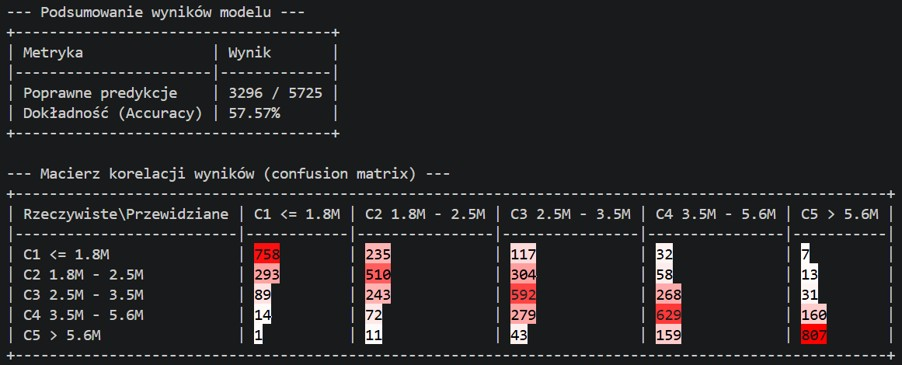
\includegraphics[width=1.0\textwidth]{img/knn-matrix.jpg}
		\caption{Macierz pomyłek dla KNN.}
		\label{fig:wyniki_knn}
	\end{figure}
	
	
	\newpage
	\subsubsection*{Naiwny Bayes}
	Model \texttt{Naiwny Bayes} został wytrenowany w dwóch wariantach -- z założeniem rozkładu Gaussa oraz z mieszaną funkcją prawdopodobieństwa, dobraną na podstawie analizy danych. Zastosowano 3 typy rozkładów prawdopodobieństwa w zależności od kolumn.
	\begin{itemize}
		\item \textbf{Rozkład ciągły} -- Klasyczny rozkład Gaussa. Czasem niezbędne okazało się wykorzystanie funkcji logarytmu, aby zbliżyć taki rozkład do rozkładu normalnego. Obliczana gęstość prawdopodobieństwa dla krzywej dzwonowej.
		\item \textbf{Rozkład multinomial (dyskretny)} -- Dane dyskretne. Prawdopodobieństwo obliczane w sposób klasyczny.
		\item \textbf{Rozkład Bernouliego (prawda / fałsz)} -- Szczególny przypadek rozkładu dyskretnego. Prawdopodobieństwo obliczane w sposób klasyczny.
	\end{itemize}
	
	Model osiągnął skuteczności kolejno 39.61\% oraz 57.16\%. Przy drugiej próbie zaszła poprawa wynosząca Z punktów procentowych, co dowodzi wyższości tej metody nad pierwszą.
	
	\begin{figure}[htbp]
		\centering
		\includegraphics[width=0.8\textwidth]{img/wyniki\_naive\_bayes\_1.png}
		\caption{Macierz pomyłek dla Naive Bayes (założenie rozkładu Gaussa).}
		\label{fig:wyniki_naive_bayes_1}
	\end{figure}
	
	\begin{figure}[htbp]
		\centering
		\includegraphics[width=0.8\textwidth]{img/wyniki\_naive\_bayes\_2.png}
		\caption{Macierz pomyłek dla Naive Bayes (założenie rozkładu mieszanego).}
		\label{fig:wyniki_naive_bayes_2}
	\end{figure}
	
	
	\newpage
	\subsubsection*{Drzewo decyzyjne}
Model \texttt{Drzewa Decyzyjnego} został zbudowany z maksymalną głębokością 13 poziomów oraz minimalną liczbą próbek w liściu równą 10. Ze względu na rozmiar zbioru treningowego podczas uczenia losowo próbkuje się co najwyżej 5~000 przykładów (stałe ziarno losowości $= 42$), co ogranicza czas budowy drzewa.

Jako kryterium podziału zastosowano indeks Giniego. Węzły obsługują dwa rodzaje podziałów, dobierane automatycznie na podstawie typu cechy.
\begin{itemize}
    \item \textbf{Podział progowy (cechy ciągłe)} -- Sprawdzany warunek \texttt{val} $\leq$ \texttt{threshold}; próg wyznaczany jest jako punkt środkowy między dwiema sąsiednimi wartościami sortowanymi rosnąco. Dla powierzchni mieszkania oraz powierzchni kuchni zastosowano transformację logarytmiczną.
    \item \textbf{Podział równościowy (cechy kategoryczne)} -- Sprawdzany warunek \texttt{val} $==$ \texttt{cat\_val}; iteracja po wszystkich unikalnych wartościach danej cechy (region, typ budynku).
\end{itemize}

Model osiągnął skuteczność 54\%.

    	\begin{figure}[htbp]
    		\centering
    		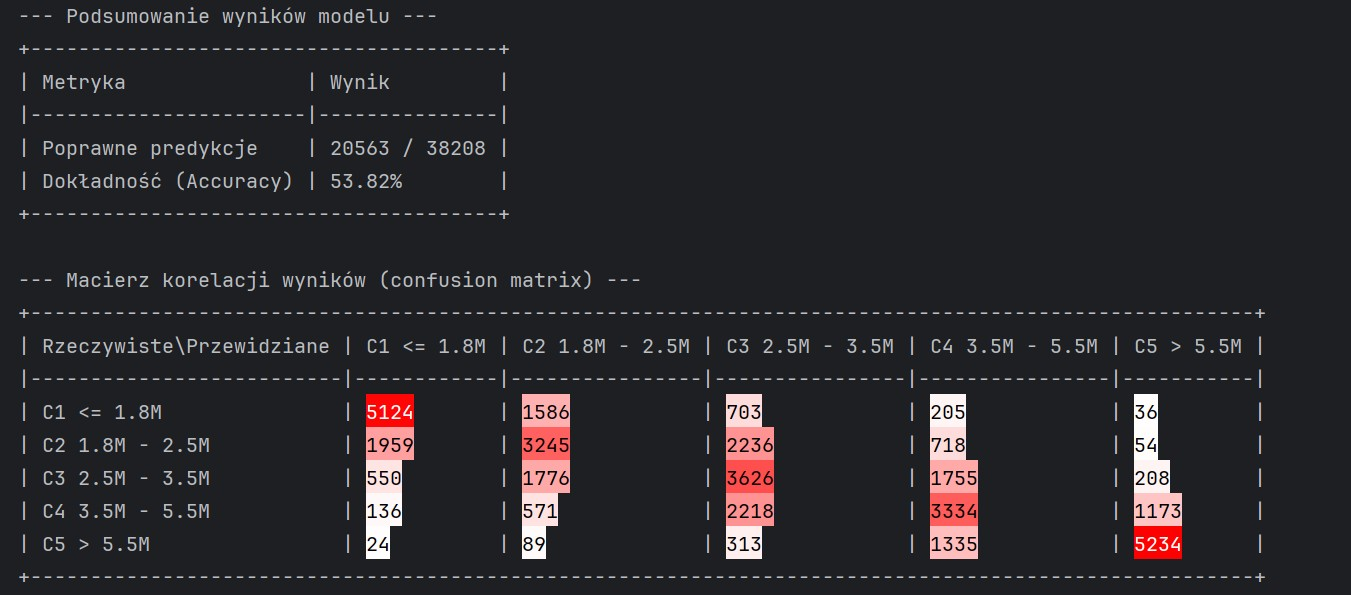
\includegraphics[width=0.8\textwidth]{img/drzewko-matrix.jpg}
    		\caption{Macierz pomyłek dla drzewa decyzyjnego.}
    		\label{fig:drzewko}
    	\end{figure}
	
	
	\newpage
	\subsection*{Porównanie}
    

    \textbf{K-Najbliższych Sąsiadów (KNN)} wyróżnia się niestandardową funkcją odległości łączącą heterogeniczne typy cech w jedną miarę -- odległość euklidesową dla wartości ciągłych (znormalizowaną odchyleniem standardowym) uzupełniono stałymi karami dla cech binarnych i kategorycznych. Predykcja opiera się na ważonym głosowaniu, w którym bliżsi sąsiedzi mają proporcjonalnie większy wpływ na wynik. Wadą modelu jest konieczność przechowywania całego zbioru treningowego w pamięci oraz liniowy czas predykcji względem jego rozmiaru. Dobór wag kar ($0{,}4$ / $0{,}5$ / $1{,}0$) ma charakter heurystyczny i nie wynika z analizy danych.
    
    \bigskip
    
    \textbf{Naiwny Bayes} osiągnął najwyższą skuteczność dzięki trafnemu dopasowaniu rozkładów prawdopodobieństwa do charakteru każdej cechy. Kluczową decyzją projektową było potraktowanie cech pozornie ciągłych (rok, miesiąc, piętro, liczba pięter, liczba pokoi, region) jako kategorycznych z rozkładem Multinomial -- co odpowiada rzeczywistości, gdyż przyjmują one skończoną liczbę wartości. Jedynie powierzchnia i powierzchnia kuchni modelowane są rozkładem Gaussa po transformacji logarytmicznej. Współrzędne geograficzne dyskretyzowane są do siatki $11 \times 11$~km, co pozwala grupować przestrzennie bliskie ogłoszenia bez obliczania rzeczywistych odległości. Całość wspomagana jest wygładzaniem Laplace'a (eliminacja problemu zerowych prawdopodobieństw) oraz wygładzaniem wariancji globalnej dla cech ciągłych. Obliczenia prowadzone w przestrzeni logarytmicznej zapobiegają niedopełnieniu arytmetycznemu.
    
    \bigskip
    
    \textbf{Drzewo Decyzyjne} jako jedyny model potrafi natywnie obsłużyć cechy kategoryczne poprzez podział równościowy, bez konieczności kodowania numerycznego. Kryterium podziału oparte na indeksie Giniego pozwala na automatyczny dobór najistotniejszych cech na każdym poziomie drzewa. Ograniczeniem jest jednak konieczność losowego próbkowania zbioru treningowego do 5~000 przykładów, co powoduje utratę informacji. Drzewo buduje twarde granice decyzyjne, które słabo uogólniają się na dane z dużą liczbą unikalnych wartości kategorycznych (np.\ identyfikator regionu z setkami wartości).

	\newpage
	\subsection{Wnioski}

	Na podstawie wygenerowanych histogramów z nakładaną krzywą Gaussa stwierdzono:
	\begin{itemize}
		\item Cechy \texttt{area} i \texttt{kitchen\_area} -- po logarytmowaniu przybliżają rozkład normalny; traktowane gaussowsko.
		\item Cechy \texttt{geo\_lat}, \texttt{geo\_lon} -- wyraźny rozkład wielomodalny (skupiska miast); traktowane jako kategorie przez spatial hashing.
		\item Cechy \texttt{publish\_month} -- rozkład cykliczny; traktowane jako kategorie.
		\item Cechy \texttt{level}, \texttt{levels}, \texttt{rooms} -- wartości dyskretne; traktowane wielomianowo.
	\end{itemize}
	
	Na podstawie wyników eksperymentów stwierdzono:
	\begin{itemize}
		\item W praktyce, najlepszym z wytrenowanych klasyfikatorów okazał się Naiwny Bayes ze względu na swoją wysoką wydajność oraz skuteczność, a także brak problemów z treningiem, biorącym pod uwagę cały zbiór danych wejściowych.
		\item KNN ze względu na swoją bardzo niską wydajność, pomimo osiągnięcia najwyższej dokładności, w praktycznych zastosowaniach byłby bezuzyteczny.
	\end{itemize}

	\newpage

	%--------------------------------------------------------------
	\section*{Pełen kod aplikacji}
	%--------------------------------------------------------------
	
	\subsubsection*{main.py}
	\begin{lstlisting}
		import os
		from utils import Utils
		from russian_flat import RussianFlat
		from preprocessor import Preprocessor
		from data_analysis import DataAnalysis
		from base_model import BaseModel
		from dummy_model import DummyModel
		from knn import Knn
		from naive_bayes import NaiveBayes
		from decision_tree import DecisionTree
		
		BORDER = 60 * "-"
		
		DATAFILE = "filtered_v3.csv"
		EXPECTED_ROWS = 200000
		
		OUT_DIR_RAW = "output_raw/"
		OUT_DIR_CLEAN = "output_clean/"
		
		NUM_BINS = 5
		
		# currently trained model
		current_model: BaseModel = DummyModel()
		
		# collected data
		raw_flats: list[RussianFlat]
		clean_flats: list[RussianFlat]
		training_data: list[RussianFlat]
		test_data: list[RussianFlat]
		
		def pause(clear: bool = False):
		print("Nacisnij Enter, aby kontynuowac...")
		input()
		if clear:
		os.system("cls" if os.name == "nt" else "clear")
		
		def menu() -> bool:
		global current_model
		
		print(BORDER)
		print("Obecnie wytrenowany model: " + current_model.name())
		print(BORDER)
		print("1 - Uruchom analize danych")
		print("2 - Trenuj model (KNN)")
		print("3 - Trenuj model (Naiwny Bayes)")
		print("4 - Trenuj model (Drzewo decyzyjne)")
		print("5 - Uruchom analize modelu (" + current_model.name() + ")")
		print("6 - Zakoncz program")
		choice = input("> ")
		
		def train_and_report(model):
		global current_model
		current_model = model
		current_model.train(training_data)
		print(f"Model {current_model.name()} wytrenowany.")
		
		if choice == "1":
		DataAnalysis.analyse_data(raw_flats, OUT_DIR_RAW)
		DataAnalysis.analyse_data(clean_flats, OUT_DIR_CLEAN)
		if choice == "2": train_and_report(Knn())
		if choice == "3": train_and_report(NaiveBayes())
		if choice == "4": train_and_report(DecisionTree())
		if choice == "5": DataAnalysis.analyse_results(
		[current_model.predict(flat.data) for flat in test_data], # predictions
		[flat.price_range for flat in test_data] # real price ranges
		)
		
		abort = choice == "6"
		if not abort:
		pause(clear=True)
		
		return not abort
		
		def main():
		global raw_flats, clean_flats, training_data, test_data
		
		print(BORDER)
		print("Rozpoczeto wstepne przetwarzanie danych...")
		
		raw_flats = RussianFlat.from_csv_file(DATAFILE, skip=1, num_bins=NUM_BINS)
		print(f"Zaladowano mieszkania w liczbie {len(raw_flats)}.")
		
		if len(raw_flats) < EXPECTED_ROWS:
		print(f"UWAGA: Oczekiwano {EXPECTED_ROWS} wierszy, ale zaladowano {len(raw_flats)}.")
		
		if len(raw_flats) > EXPECTED_ROWS:
		raw_flats = raw_flats[:EXPECTED_ROWS]
		print(f"UWAGA: Zaladowano wiecej wierszy niz oczekiwano. Uzyto tylko pierwszych {EXPECTED_ROWS} wierszy.")
		
		if len(raw_flats) == 0:
		print("Nie mozna kontynuowac bez danych. Zamykam program.")
		return
		
		outlier_indexes = Preprocessor.outlier_indexes([flat.data for flat in raw_flats])
		delete_count = len(outlier_indexes)
		delete_ratio = (delete_count / len(raw_flats)) * 100
		print(f"Zidentyfikowano {len(outlier_indexes)} outlierow ({delete_ratio:.2f}%).")
		
		clean_flats = Utils.list_without_indexes(raw_flats, outlier_indexes)
		print(f"Usunieto outliery. Pozostalo {len(clean_flats)} mieszkan.")
		
		training_data, test_data = Preprocessor.divide_data_randomly(clean_flats, ratio=0.8)
		print(f"Podzielono na zbiory treningowy ({len(training_data)}) oraz testowy ({len(test_data)}).")
		
		pause(clear=True)
		
		while menu():
		pass
		
		if __name__ == "__main__":
		main()
	\end{lstlisting}
	
	\subsubsection*{base\_model.py}
	\begin{lstlisting}
		from abc import ABC, abstractmethod
		from russian_flat import RussianFlat, RussianFlatProps
		
		class BaseModel(ABC):
		def name(self) -> str:
		return self.__class__.__name__
		
		@abstractmethod
		def train(self, training_data: list[RussianFlat]):
		pass
		
		@abstractmethod
		def predict(self, entry: RussianFlatProps) -> str:
		pass
	\end{lstlisting}
	
	\subsubsection*{data\_analysis.py}
	\begin{lstlisting}
		import os
		import shutil
		import statistics
		import matplotlib
		import math
		matplotlib.use("Agg")
		import matplotlib.pyplot as plt
		from russian_flat import RussianFlat
		from table_builder import TableBuilder
		from utils import Utils
		
		class DataAnalysis:
		
		@staticmethod
		def analyse_data(data: list[RussianFlat], output_dir: str):
		if not data:
		print("Brak danych do analizy.")
		return
		
		# 1. Zarzadzanie katalogiem wyjsciowym
		if os.path.exists(output_dir):
		shutil.rmtree(output_dir)
		os.makedirs(output_dir)
		
		# 2. Analiza rozkladu klas cenowych
		print(f"\n--- Analiza danych ({output_dir}) - liczba rekordow: {len(data)} ---")
		distribution = {}
		for flat in data:
		price_range = flat.price_range
		distribution[price_range] = distribution.get(price_range, 0) + 1
		
		builder_dist = TableBuilder(["Przedzial cenowy", "Liczba mieszkan", "Procentowo"])
		total = len(data)
		for price_range, count in sorted(distribution.items()):
		percentage = (count / total) * 100
		builder_dist.add_row([price_range, count, f"{percentage:.1f}%"])
		print(builder_dist.build())
		
		# POBRANIE CECH CIAGLYCH
		continuous_names = [
		field for field in Utils.get_attrs_of(data[0].data, (int, float))
		if type(getattr(data[0].data, field)) is not bool
		]
		
		# 3. Analiza statystyczna cech ciaglych
		print("\n--- Statystyki cech ciaglych ---")
		builder_stats = TableBuilder(["Cecha", "Min", "Max", "Srednia", "Odch. Stand."])
		for field in continuous_names:
		values = [getattr(entry.data, field) for entry in data]
		min_v = round(min(values), 4)
		max_v = round(max(values), 4)
		avg_v = round(statistics.mean(values), 4)
		stdev_v = round(statistics.stdev(values), 4) if len(values) > 1 else 0.0
		builder_stats.add_row([field, min_v, max_v, avg_v, stdev_v])
		print(builder_stats.build())
		
		# 4. MACIERZ KORELACJI (Pearson)
		print("\n--- Macierz Korelacji (Cechy ciagle) ---")
		
		def color_by_corr(value: float, text: str) -> str:
		value = max(-1.0, min(1.0, value))
		intensity = abs(value)
		base = int(255 * (1 - intensity))
		if value >= 0:
		r, g, b = 255, base, base
		else:
		r, g, b = base, base, 255
		brightness = 0.299 * r + 0.587 * g + 0.114 * b
		fg = 30 if brightness > 128 else 97
		return f"\x1b[{fg}m\x1b[48;2;{r};{g};{b}m{text}\x1b[0m"
		
		builder_corr = TableBuilder(["Cecha"] + continuous_names)
		
		for f1 in continuous_names:
		row = [f1]
		vals1 = [getattr(entry.data, f1) for entry in data]
		
		for f2 in continuous_names:
		vals2 = [getattr(entry.data, f2) for entry in data]
		
		if f1 == f2:
		row.append(color_by_corr(1.0, "1.00"))
		else:
		try:
		corr = statistics.correlation(vals1, vals2)
		row.append(color_by_corr(corr, f"{corr:.2f}"))
		except statistics.StatisticsError:
		row.append("N/A")
		
		builder_corr.add_row(row)
		
		print(builder_corr.build())
		
		# 5. Wykresy
		print("\n--- Generowanie wykresow ---")
		try:
		# Wykres rozkladu klas cenowych
		fig, ax = plt.subplots(figsize=(8, 5))
		ranges = [price_range for price_range, _ in sorted(distribution.items())]
		counts = [distribution[price_range] for price_range in ranges]
		ax.bar(ranges, counts, color="#4c72b0")
		ax.set_xlabel("Przedzial cenowy")
		ax.set_ylabel("Liczba mieszkan")
		ax.set_title("Rozklad liczby mieszkan wedlug przedzialow cenowych")
		ax.set_xticks(range(len(ranges)))
		ax.set_xticklabels(ranges, rotation=45, ha="right")
		fig.tight_layout()
		fig.savefig(os.path.join(output_dir, "class_distribution.png"), dpi=150)
		plt.close(fig)
		
		# Wykres macierzy korelacji
		fig, ax = plt.subplots(figsize=(max(6, len(continuous_names) * 0.8), max(6, len(continuous_names) * 0.8)))
		corr_matrix = []
		for f1 in continuous_names:
		row = []
		vals1 = [getattr(entry.data, f1) for entry in data]
		for f2 in continuous_names:
		vals2 = [getattr(entry.data, f2) for entry in data]
		if f1 == f2:
		row.append(1.0)
		else:
		try:
		row.append(statistics.correlation(vals1, vals2))
		except statistics.StatisticsError:
		row.append(0.0)
		corr_matrix.append(row)
		
		im = ax.imshow(corr_matrix, cmap="bwr", vmin=-1, vmax=1)
		ax.set_xticks(range(len(continuous_names)))
		ax.set_yticks(range(len(continuous_names)))
		ax.set_xticklabels(continuous_names, rotation=45, ha="right")
		ax.set_yticklabels(continuous_names)
		ax.set_title("Macierz korelacji cech ciaglych")
		fig.colorbar(im, ax=ax, label="Korelacja Pearsona")
		
		for i in range(len(continuous_names)):
		for j in range(len(continuous_names)):
		corr_value = corr_matrix[i][j]
		percent_text = f"{corr_value * 100:.0f}%"
		ax.text(j, i, percent_text,
		ha="center", va="center",
		color="black" if abs(corr_value) < 0.5 else "white",
		fontsize=8)
		
		fig.tight_layout()
		fig.savefig(os.path.join(output_dir, "correlation_matrix.png"), dpi=150)
		plt.close(fig)
		
		# 6. Wykresy rozkladu poszczegolnych cech
		print("Generowanie wykresow rozkladu poszczegolnych cech...")
		for field in continuous_names:
		values = [getattr(entry.data, field) for entry in data]
		if not values:
		continue
		
		fig, ax = plt.subplots(figsize=(8, 5))
		
		unique_values = set(values)
		is_discrete = len(unique_values) <= 25 or all(isinstance(v, int) or (isinstance(v, float) and v.is_integer()) for v in values)
		
		if is_discrete:
		counts = {}
		for v in values:
		counts[v] = counts.get(v, 0) + 1
		
		x_vals = sorted(counts.keys())
		
		total_count = len(values)
		y_vals = [counts[x] / total_count for x in x_vals]
		
		ax.bar(x_vals, y_vals, color="#2a9d8f", edgecolor="black", alpha=0.7, label="Wartosci (rzeczywistosc)")
		
		if len(x_vals) <= 15:
		ax.set_xticks(x_vals)
		else:
		step = len(x_vals) // 15
		ax.set_xticks(x_vals[::step])
		
		ax.set_title(f"Rozklad wartosci dyskretnej: {field}")
		else:
		ax.hist(values, bins=30, density=True, color="#e9c46a", edgecolor="black", alpha=0.6, label="Histogram (rzeczywistosc)")
		ax.set_title(f"Rozklad wartosci ciaglej: {field}")
		
		if len(values) > 1:
		mean = statistics.mean(values)
		stdev = statistics.stdev(values)
		
		if stdev > 0:
		x_min, x_max = min(values), max(values)
		step = (x_max - x_min) / 100 if x_max > x_min else 1
		x_axis = [x_min + i * step for i in range(101)]
		y_axis = []
		for x in x_axis:
		exponent = math.exp(-0.5 * ((x - mean) / stdev) ** 2)
		pdf = (1 / (stdev * math.sqrt(2 * math.pi))) * exponent
		y_axis.append(pdf)
		
		ax.plot(x_axis, y_axis, color="#e76f51", linewidth=2, label="Krzywa Gaussa (zalozenie modelu)")
		ax.legend()
		
		ax.set_ylabel("Czestosc / Gestosc prawdopodobienstwa")
		ax.set_xlabel(field)
		fig.tight_layout()
		safe_name = field.replace(" ", "_").replace("/", "_")
		fig.savefig(os.path.join(output_dir, f"dist_{safe_name}.png"), dpi=150)
		plt.close(fig)
		
		print(f"Wykresy zapisane do katalogu: \"{output_dir}\".")
		except Exception as e:
		print("Blad przy generowaniu wykresow:", e)
		
		print("\nAnaliza danych zakonczona.")
		
		@staticmethod
		def analyse_results(predicted: list[str], real: list[str]):
		if not predicted or not real or len(predicted) != len(real):
		print("Blad: Dane przewidywane i rzeczywiste nie pasuja do siebie.")
		return
		
		print("\n--- Podsumowanie wynikow modelu ---")
		correct = sum(1 for p, r in zip(predicted, real) if p == r)
		total = len(predicted)
		accuracy = (correct / total) * 100
		
		builder = TableBuilder(["Metryka", "Wynik"])
		builder.add_row(["Poprawne predykcje", f"{correct} / {total}"])
		builder.add_row(["Dokladnosc (Accuracy)", f"{accuracy:.2f}%"])
		print(builder.build())
		
		print("\n--- Macierz korelacji wynikow (confusion matrix) ---")
		labels = sorted(set(real) | set(predicted))
		confusion = {real_label: {pred_label: 0 for pred_label in labels} for real_label in labels}
		for p, r in zip(predicted, real):
		confusion[r][p] += 1
		
		max_count = max(
		confusion[r][p]
		for r in labels
		for p in labels
		) if labels else 0
		
		def color_by_value(count: int, text: str) -> str:
		intensity = count / max_count if max_count else 0.0
		base = int(255 * (1 - intensity))
		r, g, b = 255, base, base
		brightness = 0.299 * r + 0.587 * g + 0.114 * b
		fg = 30 if brightness > 128 else 97
		return f"\x1b[{fg}m\x1b[48;2;{r};{g};{b}m{text}\x1b[0m"
		
		builder_conf = TableBuilder(["Rzeczywiste\\Przewidziane"] + labels)
		for real_label in labels:
		row = [real_label]
		for pred_label in labels:
		count = confusion[real_label][pred_label]
		row.append(color_by_value(count, str(count)))
		builder_conf.add_row(row)
		print(builder_conf.build())
		
		print("Analiza wynikow modelu zakonczona.")
	\end{lstlisting}
	
	\subsubsection*{decision\_tree.py}
	\begin{lstlisting}
		import math
		import random
		from collections import Counter
		from russian_flat import RussianFlat, RussianFlatProps
		from base_model import BaseModel
		
		MAX_TRAIN_SAMPLES = 5_000
		MAX_DEPTH = 13
		MIN_SAMPLES_LEAF = 10
		
		class _Node:
		__slots__ = ('feat', 'threshold', 'cat_val', 'is_cat', 'left', 'right', 'label')
		
		def __init__(self):
		self.feat = None
		self.threshold = None
		self.cat_val = None
		self.is_cat = False
		self.left = None
		self.right = None
		self.label = None
		
		class DecisionTree(BaseModel):
		def __init__(self, max_depth: int = MAX_DEPTH, min_samples: int = MIN_SAMPLES_LEAF):
		self.max_depth = max_depth
		self.min_samples = min_samples
		self.root: _Node | None = None
		
		def name(self) -> str:
		return "Drzewo decyzyjne"
		
		def train(self, training_data: list[RussianFlat]):
		print(f"Trenuje drzewo na {min(len(training_data), MAX_TRAIN_SAMPLES)} probkach...")
		if len(training_data) > MAX_TRAIN_SAMPLES:
		data = random.Random(42).sample(training_data, MAX_TRAIN_SAMPLES)
		else:
		data = list(training_data)
		
		X = [_extract(flat.data) for flat in data]
		y = [flat.price_range for flat in data]
		self.root = self._build(X, y, 0)
		
		def predict(self, entry: RussianFlatProps) -> str:
		if self.root is None:
		return "unknown"
		return _traverse(self.root, _extract(entry))
		
		def _build(self, X: list, y: list, depth: int) -> _Node:
		node = _Node()
		counts = Counter(y)
		node.label = counts.most_common(1)[0][0]
		
		if depth >= self.max_depth or len(y) <= self.min_samples or len(counts) == 1:
		return node
		
		best = self._best_split(X, y, len(y))
		if best is None:
		return node
		
		feat, threshold, cat_val, is_cat = best
		node.feat = feat
		node.threshold = threshold
		node.cat_val = cat_val
		node.is_cat = is_cat
		
		if is_cat:
		mask = [x[feat] == cat_val for x in X]
		else:
		mask = [x[feat] <= threshold for x in X]
		
		X_l = [x for x, m in zip(X, mask) if m]
		y_l = [lbl for lbl, m in zip(y, mask) if m]
		X_r = [x for x, m in zip(X, mask) if not m]
		y_r = [lbl for lbl, m in zip(y, mask) if not m]
		
		if not X_l or not X_r:
		return node
		
		node.left = self._build(X_l, y_l, depth + 1)
		node.right = self._build(X_r, y_r, depth + 1)
		node.label = None
		return node
		
		def _best_split(self, X: list, y: list, n: int):
		base_gini = _gini_counter(Counter(y), n)
		best_gain = 1e-10
		best = None
		
		for feat in range(len(X[0])):
		vals = [x[feat] for x in X]
		
		if isinstance(vals[0], str):
		for cat_val in set(vals):
		l_labels = [lbl for v, lbl in zip(vals, y) if v == cat_val]
		r_labels = [lbl for v, lbl in zip(vals, y) if v != cat_val]
		nl, nr = len(l_labels), len(r_labels)
		if nl < self.min_samples or nr < self.min_samples:
		continue
		gain = base_gini - (nl / n * _gini(l_labels) + nr / n * _gini(r_labels))
		if gain > best_gain:
		best_gain = gain
		best = (feat, None, cat_val, True)
		else:
		pairs = sorted(zip(vals, y))
		right_cnt = Counter(y)
		left_cnt: Counter = Counter()
		nl, nr = 0, n
		prev = None
		
		for val, lbl in pairs:
		if prev is not None and val != prev and nl >= self.min_samples and nr >= self.min_samples:
		gain = base_gini - (
		nl / n * _gini_counter(left_cnt, nl) +
		nr / n * _gini_counter(right_cnt, nr)
		)
		if gain > best_gain:
		best_gain = gain
		best = (feat, (prev + val) / 2.0, None, False)
		left_cnt[lbl] += 1
		right_cnt[lbl] -= 1
		if right_cnt[lbl] == 0:
		del right_cnt[lbl]
		nl += 1
		nr -= 1
		prev = val
		
		return best
		
		
		def _gini_counter(counter: Counter, n: int) -> float:
		if n == 0:
		return 0.0
		return 1.0 - sum((c / n) ** 2 for c in counter.values())
		
		def _gini(labels: list) -> float:
		n = len(labels)
		if n == 0:
		return 0.0
		return 1.0 - sum((c / n) ** 2 for c in Counter(labels).values())
		
		def _extract(entry: RussianFlatProps) -> list:
		return [
		math.log(float(entry.area) + 1e-5),
		math.log(float(entry.kitchen_area) + 1e-5),
		float(entry.geo_lat),
		float(entry.geo_lon),
		float(entry.level),
		float(entry.levels),
		float(entry.rooms),
		float(entry.publish_year),
		float(entry.publish_month),
		1.0 if entry.new_building else 0.0,
		float(entry.region_id),
		str(entry.building_type),
		]
		
		def _traverse(node: _Node, features: list) -> str:
		if node.label is not None:
		return node.label
		val = features[node.feat]
		go_left = (val == node.cat_val) if node.is_cat else (val <= node.threshold)
		return _traverse(node.left if go_left else node.right, features)
	\end{lstlisting}
	
	\subsubsection*{dummy\_model.py}
	\begin{lstlisting}
		from russian_flat import RussianFlat, RussianFlatProps
		from base_model import BaseModel
		
		class DummyModel(BaseModel):
		def train(self, training_data: list[RussianFlat]):
		pass
		
		def predict(self, entry: RussianFlatProps) -> str:
		return "unknown"
	\end{lstlisting}
	
	\subsubsection*{knn.py}
	\begin{lstlisting}
		import math
		import statistics
		from russian_flat import RussianFlat, RussianFlatProps
		from base_model import BaseModel
		
		class Knn(BaseModel):
		def __init__(self, k: int = 7):
		self.k = k
		self.training_data: list[RussianFlat] = []
		self.continuous_scales: tuple[float, ...] = ()
		
		def train(self, training_data: list[RussianFlat]):
		self.training_data = training_data[:]
		self.continuous_scales = self._compute_continuous_scales(self.training_data)
		
		def predict(self, entry: RussianFlatProps) -> str:
		if not self.training_data:
		return "unknown"
		
		entry_features = self._extract_features(entry)
		distances = []
		
		for flat in self.training_data:
		train_features = self._extract_features(flat.data)
		dist = self._distance(entry_features, train_features)
		distances.append((dist, flat.price_range))
		
		distances.sort(key=lambda item: item[0])
		nearest = distances[: self.k]
		
		if not nearest:
		return "unknown"
		
		return self._vote(nearest)
		
		def _vote(self, neighbors: list[tuple[float, str]]) -> str:
		weights: dict[str, float] = {}
		for dist, label in neighbors:
		if dist <= 1e-9:
		return label
		weights[label] = weights.get(label, 0.0) + 1.0 / (dist + 1e-9)
		
		return max(weights.items(), key=lambda item: item[1])[0]
		
		def _distance(
		self,
		first: tuple[tuple[float, ...], bool, str, str],
		second: tuple[tuple[float, ...], bool, str, str],
		) -> float:
		first_cont, first_new_building, first_region, first_building = first
		second_cont, second_new_building, second_region, second_building = second
		
		squared_sum = 0.0
		for value_a, value_b, scale in zip(first_cont, second_cont, self.continuous_scales):
		diff = (value_a - value_b) / scale
		squared_sum += diff * diff
		
		numeric_distance = math.sqrt(squared_sum)
		
		binary_distance = 0.4 if first_new_building != second_new_building else 0.0
		region_distance = 1.0 if first_region != second_region else 0.0
		building_distance = 0.5 if first_building != second_building else 0.0
		
		return numeric_distance + binary_distance + region_distance + building_distance
		
		def _compute_continuous_scales(self, training_data: list[RussianFlat]) -> tuple[float, ...]:
		if not training_data:
		return (1.0,) * 9
		
		examples = [_ for _ in training_data]
		columns = list(zip(*(self._extract_features(flat.data)[0] for flat in examples)))
		
		scales: list[float] = []
		for column in columns:
		stdev = statistics.stdev(column) if len(column) > 1 else 0.0
		if stdev <= 0.0:
		stdev = 1.0
		scales.append(stdev)
		
		return tuple(scales)
		
		@staticmethod
		def _extract_features(entry: RussianFlatProps) -> tuple[tuple[float, ...], bool, str, str]:
		lat_km = float(entry.geo_lat) * 111.0
		lon_km = float(entry.geo_lon) * 111.0 * math.cos(math.radians(float(entry.geo_lat)))
		
		continuous = (
		float(entry.publish_year),
		float(entry.publish_month),
		float(entry.level),
		float(entry.levels),
		float(entry.rooms),
		math.log(float(entry.area) + 1e-5),
		math.log(float(entry.kitchen_area) + 1e-5),
		lat_km,
		lon_km,
		)
		
		return continuous, entry.new_building, entry.region_id, entry.building_type
	\end{lstlisting}
	
	\subsubsection*{naive\_bayes.py}
	\begin{lstlisting}
		import math
		from collections import defaultdict
		from russian_flat import RussianFlat, RussianFlatProps
		from base_model import BaseModel
		
		class NaiveBayes(BaseModel):
		def __init__(self):
		self.class_counts = defaultdict(int)
		self.class_priors = {}
		
		self.continuous_stats = defaultdict(list)
		self.binary_probs = defaultdict(list)
		self.cat_probs = defaultdict(dict)
		self.cat_unseen_probs = defaultdict(dict)
		
		self.num_classes = 0
		
		def train(self, training_data: list[RussianFlat]):
		separated_data_cont = defaultdict(list)
		separated_data_bin = defaultdict(list)
		separated_data_cat = defaultdict(list)
		
		all_continuous_features = []
		global_cat_uniques = defaultdict(set)
		
		total_samples = len(training_data)
		
		# 1. Zbieranie i grupowanie danych
		for flat in training_data:
		label = flat.price_range
		cont_features, bin_features, cat_features = self.extract_features(flat.data)
		
		separated_data_cont[label].append(cont_features)
		separated_data_bin[label].append(bin_features)
		separated_data_cat[label].append(cat_features)
		all_continuous_features.append(cont_features)
		self.class_counts[label] += 1
		
		for i, val in enumerate(cat_features):
		global_cat_uniques[i].add(val)
		
		self.num_classes = len(self.class_counts)
		
		# 2. Obliczanie globalnego wygladzania wariancji dla cech ciaglych
		global_variances = []
		if total_samples > 1 and all_continuous_features:
		global_columns = list(zip(*all_continuous_features))
		for col in global_columns:
		mean = sum(col) / len(col)
		var = sum((x - mean) ** 2 for x in col) / (len(col) - 1)
		global_variances.append(var)
		else:
		global_variances = [0.0] * len(all_continuous_features[0])
		
		epsilons = [max(1e-4 * var, 1e-9) for var in global_variances]
		
		# 3. Trening parametrow dla kazdej klasy
		for label in self.class_counts:
		self.class_priors[label] = (self.class_counts[label] + 1) / (total_samples + self.num_classes)
		class_size = self.class_counts[label]
		
		# 1. Trening: Ciagle (Gauss)
		cont_columns = zip(*separated_data_cont[label])
		cont_stats = []
		for i, column in enumerate(cont_columns):
		mean = sum(column) / len(column)
		if len(column) > 1:
		variance = sum((x - mean) ** 2 for x in column) / (len(column) - 1)
		else:
		variance = 0.0
		cont_stats.append((mean, variance + epsilons[i]))
		self.continuous_stats[label] = cont_stats
		
		# 2. Trening: Binarne (Bernoulli)
		bin_columns = zip(*separated_data_bin[label])
		bin_probs = []
		alpha_bin = 1.0
		for column in bin_columns:
		ones_count = sum(column)
		prob_one = (ones_count + alpha_bin) / (class_size + 2 * alpha_bin)
		bin_probs.append(prob_one)
		self.binary_probs[label] = bin_probs
		
		# 3. Trening: Kategoryczne (Multinomial)
		cat_columns = zip(*separated_data_cat[label])
		self.cat_probs[label] = {}
		self.cat_unseen_probs[label] = {}
		alpha_cat = 1.0
		
		for i, column in enumerate(cat_columns):
		counts = defaultdict(int)
		for val in column:
		counts[val] += 1
		
		v_total = len(global_cat_uniques[i])
		self.cat_probs[label][i] = {}
		
		for val in global_cat_uniques[i]:
		prob = (counts[val] + alpha_cat) / (class_size + alpha_cat * v_total)
		self.cat_probs[label][i][val] = prob
		
		self.cat_unseen_probs[label][i] = alpha_cat / (class_size + alpha_cat * v_total)
		
		def predict(self, entry: RussianFlatProps) -> str:
		cont_features, bin_features, cat_features = self.extract_features(entry)
		
		best_label = "unknown"
		max_log_prob = -float('inf')
		
		for label in self.class_counts:
		log_prob = math.log(self.class_priors[label])
		
		# 1. Ciagle (Gauss)
		stats = self.continuous_stats[label]
		for x, (mean, var) in zip(cont_features, stats):
		log_pdf = -0.5 * math.log(2 * math.pi * var) - ((x - mean) ** 2) / (2 * var)
		log_prob += log_pdf
		
		# 2. Binarne (Bernoulli)
		probs = self.binary_probs[label]
		for x, p_one in zip(bin_features, probs):
		if x == 1.0:
		log_prob += math.log(p_one)
		else:
		log_prob += math.log(1.0 - p_one)
		
		# 3. Kategoryczne (Multinomial)
		for i, val in enumerate(cat_features):
		prob = self.cat_probs[label][i].get(val, self.cat_unseen_probs[label][i])
		log_prob += math.log(prob)
		
		if log_prob > max_log_prob:
		max_log_prob = log_prob
		best_label = label
		
		return best_label
		
		@staticmethod
		def extract_features(entry: RussianFlatProps) -> tuple[tuple[float, ...], tuple[float, ...], tuple]:
		continuous = (
		math.log(float(entry.area) + 1e-5), 
		math.log(float(entry.kitchen_area) + 1e-5),
		)
		
		binary = (
		1.0 if entry.new_building else 0.0,
		)
		
		categorical = (
		int(entry.publish_year),
		int(entry.publish_month),
		int(entry.level),
		int(entry.levels),
		int(entry.rooms),
		int(entry.region_id),
		str(entry.building_type),
		f"{round(float(entry.geo_lat), 1)}_{round(float(entry.geo_lon), 1)}", # 11km x 11km
		)
		
		return continuous, binary, categorical
	\end{lstlisting}
	
	\subsubsection*{preprocessor.py}
	\begin{lstlisting}
		from utils import Utils
		from typing import NamedTuple
		from operator import attrgetter
		from typing import Callable
		import statistics
		import random
		
		class Preprocessor:
		
		@staticmethod
		def outlier_indexes(data: list) -> list[int]:
		if len(data) <= 1:
		return []
		
		continuous_names = Utils.get_attrs_of(data[0], (int, float))
		getters = {f: attrgetter(f) for f in continuous_names}
		
		means = {
			field: statistics.mean(getters[field](entry) for entry in data)
			for field in continuous_names
		}
		
		stdevs = {
			field: statistics.stdev(getters[field](entry) for entry in data)
			for field in continuous_names
		}
		
		def is_outlier(entry) -> bool:
		return any(
		abs(getters[field](entry) - means[field]) > 3 * stdevs[field]
		for field in continuous_names
		)
		
		return [i for i, entry in enumerate(data) if is_outlier(entry)]
		
		@staticmethod
		def divide_data_randomly(data: list, ratio: float) -> tuple[list, list]:
		data = data[:]
		rng = random.Random(42) # fixed seed for reproducibility
		rng.shuffle(data)
		split_index = int(len(data) * ratio)
		return data[:split_index], data[split_index:]
	\end{lstlisting}
	
	\subsubsection*{russian\_flat.py}
	\begin{lstlisting}
		import statistics
		import bisect
		from typing import NamedTuple
		from datetime import date, datetime, time
		
		class RussianFlatCsv(NamedTuple):
		price: int
		date_value: date
		time_value: time
		geo_lat: float
		geo_lon: float
		region: int
		building_type: int
		level: int
		levels: int
		rooms: int
		area: float
		kitchen_area: float
		object_type: int
		
		@staticmethod
		def from_csv_line(line: str) -> 'RussianFlatCsv':
		parts = line.strip().split(",")
		
		dt = datetime.strptime(
		f"{parts[1]} {parts[2]}",
		"%Y-%m-%d %H:%M:%S"
		)
		
		return RussianFlatCsv(
		price=int(parts[0]),
		date_value=dt.date(),
		time_value=dt.time(),
		geo_lat=float(parts[3]),
		geo_lon=float(parts[4]),
		region=int(parts[5]),
		building_type=int(parts[6]),
		level=int(parts[7]),
		levels=int(parts[8]),
		rooms=int(parts[9]),
		area=float(parts[10]),
		kitchen_area=float(parts[11]),
		object_type=int(parts[12])
		)
		
		class RussianFlatProps(NamedTuple):
		publish_year: int
		publish_month: int
		geo_lat: float
		geo_lon: float
		region_id: str
		building_type: str
		level: int
		levels: int
		rooms: int
		area: float
		kitchen_area: float
		new_building: bool
		
		class RussianFlat(NamedTuple):
		price_range: str
		data: RussianFlatProps
		
		price_dividers: list[float] = []
		
		@classmethod
		def set_price_dividers(cls, prices: list[int], num_bins: int):
		cls.price_dividers = statistics.quantiles(prices, n=num_bins)
		
		@classmethod
		def get_dynamic_price_range(cls, price: int) -> str:
		if not cls.price_dividers:
		return "unknown"
		
		divs = cls.price_dividers
		idx = bisect.bisect_right(divs, price)
		
		if idx == 0:
		return f"C{idx+1} <= {divs[0]/1_000_000:.1f}M"
		
		if idx == len(divs):
		return f"C{idx+1} > {divs[-1]/1_000_000:.1f}M"
		
		low, high = divs[idx-1], divs[idx]
		return f"C{idx+1} {low/1_000_000:.1f}M - {high/1_000_000:.1f}M"
		
		@classmethod
		def from_csv_file(cls, filename: str, skip: int, num_bins: int) -> list['RussianFlat']:
		csv_records = []
		with open(filename, "r", encoding="utf-8") as f:
		for i, line in enumerate(f):
		if i < skip:
		continue
		csv_records.append(RussianFlatCsv.from_csv_line(line))
		
		if not csv_records:
		return []
		
		all_prices = [record.price for record in csv_records]
		cls.set_price_dividers(all_prices, num_bins)
		
		flats = []
		for record in csv_records:
		flats.append(
		cls(
		price_range=cls.get_dynamic_price_range(record.price),
		data=RussianFlatProps(
		publish_year=record.date_value.year,
		publish_month=record.date_value.month,
		geo_lat=record.geo_lat,
		geo_lon=record.geo_lon,
		region_id=str(record.region),
		building_type=cls.building_type_string(record.building_type),
		level=record.level,
		levels=record.levels,
		rooms=record.rooms,
		area=record.area,
		kitchen_area=record.kitchen_area,
		new_building=record.object_type == 11
		)
		)
		)
		
		return flats
		
		@classmethod
		def from_csv_line(cls, line: str) -> 'RussianFlat':
		flat_csv = RussianFlatCsv.from_csv_line(line)
		return cls(
		price_range=cls.get_dynamic_price_range(flat_csv.price),
		data=RussianFlatProps(
		publish_year=flat_csv.date_value.year,
		publish_month=flat_csv.date_value.month,
		geo_lat=flat_csv.geo_lat,
		geo_lon=flat_csv.geo_lon,
		region_id=str(flat_csv.region),
		building_type=cls.building_type_string(flat_csv.building_type),
		level=flat_csv.level,
		levels=flat_csv.levels,
		rooms=flat_csv.rooms,
		area=flat_csv.area,
		kitchen_area=flat_csv.kitchen_area,
		new_building=flat_csv.object_type == 11
		)
		)
		
		@staticmethod
		def building_type_string(building_type: int) -> str:
		if building_type == 0: return "other"
		if building_type == 1: return "panel"
		if building_type == 2: return "monolithic"
		if building_type == 3: return "brick"
		if building_type == 4: return "block"
		if building_type == 5: return "wood"
		return "unknown"
	\end{lstlisting}
	
	\subsubsection*{table\_builder.py}
	\begin{lstlisting}
		import re
		
		class TableBuilder:
		ANSI_ESCAPE = re.compile(r"\x1b\[[0-9;]*m")
		
		def __init__(self, header: list):
		self.clen = len(header)
		self.column_widths = [0] * self.clen
		self.rowlists = []
		self.add_row(header)
		
		@staticmethod
		def _strip_ansi(text: str) -> str:
		return TableBuilder.ANSI_ESCAPE.sub("", text)
		
		def add_row(self, row: list):
		if len(row) < self.clen:
		row = row + [""] * (self.clen - len(row))
		
		self.column_widths = [
		max(self.column_widths[j], len(self._strip_ansi(str(row[j]))) )
		for j in range(self.clen)
		]
		self.rowlists.append(row)
		
		def build(self) -> str:
		result = [
		self._format_outside_sep(),
		self._format_header(),
		self._format_inside_sep()
		]
		
		for row in self.rowlists[1:]:
		result.append(self._format_row(row))
		
		result.append(self._format_outside_sep())
		return "\n".join(result)
		
		def _format_header(self) -> str:
		return self._format_row(self.rowlists[0])
		
		def _format_inside_sep(self) -> str:
		return self._format_row(["-" * self.column_widths[j] for j in range(self.clen)]).replace(" ", "-")
		
		def _format_outside_sep(self) -> str:
		return "+" + ("-" * (len(self._format_header()) - 2)) + "+"
		
		def _format_row(self, row: list) -> str:
		cells = []
		for j in range(self.clen):
		raw = str(row[j])
		visible = self._strip_ansi(raw)
		padding = self.column_widths[j] - len(visible)
		cells.append(raw + " " * padding)
		return "| " + " | ".join(cells) + " |"
	\end{lstlisting}
	
	\subsubsection*{utils.py}
	\begin{lstlisting}
		class Utils:
		
		@staticmethod
		def list_without_indexes(lst: list, indexes: list[int]) -> list:
		return [item for i, item in enumerate(lst) if i not in indexes]
		
		@staticmethod
		def get_attrs_of(record, types: tuple[type, ...]) -> list[str]:
		all_names = record._fields if hasattr(record, "_fields") else record.__dict__.keys()
		return [
		field for field in all_names
		if isinstance(getattr(record, field), types)
		]
	\end{lstlisting}
	
	\end{document}